% Compact PGFPlots panel for sampled qldpc_16_1_4_signature_cap4 BSC correction-class derivative.
% Requires \usepackage{pgfplots} and \pgfplotsset{compat=1.18}.
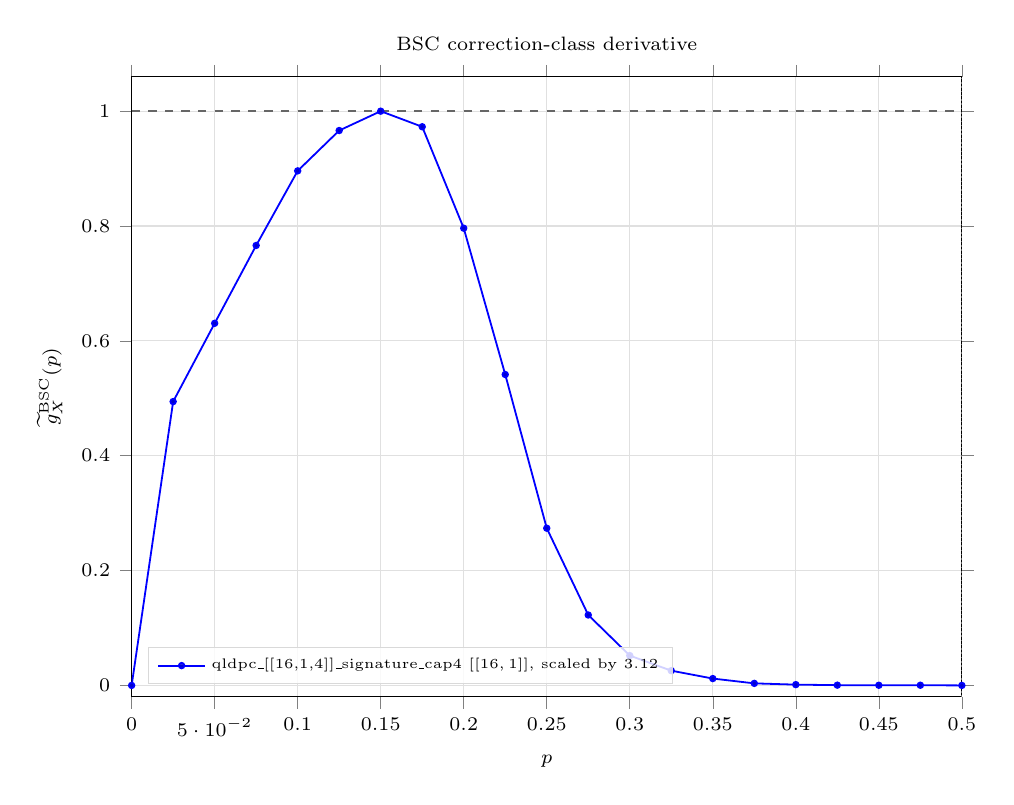
\begin{tikzpicture}
\begin{axis}[
  name=scaledBSCGEXITQldpc1614SignatureCap4Axis,
  width=\linewidth,
  height=0.78\linewidth,
  title={BSC correction-class derivative},
  title style={font=\scriptsize},
  xlabel={$p$},
  ylabel={$\widetilde g_X^{\rm BSC}(p)$},
  xmin=0, xmax=0.5,
  ymin=-0.02, ymax=1.06,
  grid=both,
  major grid style={black!12},
  minor grid style={black!6},
  tick align=outside,
  tick label style={font=\scriptsize},
  label style={font=\scriptsize},
  legend cell align={left},
  legend style={draw=black!15, fill=white, fill opacity=0.82, text opacity=1, at={(0.02,0.02)}, anchor=south west, font=\tiny},
]
\addplot[black!60, densely dotted, line width=0.55pt, forget plot] coordinates {(0.5,-0.02) (0.5,1.06)};
\addplot[black!60, dashed, line width=0.55pt, forget plot] coordinates {(0,1) (0.5,1)};
\addplot+[color=blue, mark=*, mark size=1.0pt, line width=0.65pt]
coordinates {(0,0) (0.025,0.494284266592) (0.05,0.630599100161) (0.075,0.766185142622) (0.1,0.896069225219) (0.125,0.966318317349) (0.15,1) (0.175,0.972852017844) (0.2,0.796216800432) (0.225,0.541406664622) (0.25,0.273808649318) (0.275,0.122638605922) (0.3,0.0519323790375) (0.325,0.0256890542381) (0.35,0.0119501308175) (0.375,0.00357337511253) (0.4,0.00137316040884) (0.425,0.000467860838305) (0.45,0.000266081092682) (0.475,0.000321723576183) (0.5,0)};
\addlegendentry{qldpc\_[[16,1,4]]\_signature\_cap4 $[[16,1]]$, scaled by $3.12$}
\end{axis}
\end{tikzpicture}
